% Denne fil er inkluderet i udtraekning_af_regioner.tex
{
Sløring, som kommer fra det engelske ord ``blur'', er en gruppering af
filtre som bruges til at fjerne støj og uregelmæssigheder i billeder. Vi
så i afsnit \ref{subsec_floodfill}, at metoden floodfill nogle gange kan
have svært ved at fylde hele regionen ud. Specielt i figur
\ref{dot_ff_var_7_7} ses at himlen har små huller. En sløring af
billedet kan hjælpe med at glatte farverne ud, således at vi dækker mere
af regionen. Sløring af billedet kan også hjælpe til at fjerne diverse
artefakter, såsom revner eller pletter i billedet. Specielt i
vores testbillede, der som tidligere nævnt er malet med en masse
prikker, er det en stor hjælp at sløre billedet, så farverne bliver mere
ensartede. Vi vil nu se på tre forskellige måder at opnå dette på.

De to første et såkaldte lav-pas filtre som har svært ved at bibeholde
kanterne i et billede, men arbejder til gengæld direkte på billedet. Den
tredie metode bibeholder til en vis grad kanterne bedre, men kan ikke
arbejde direkte på billedet, hvilket kræver et større pladsforbrug.

\subsubsection*{Simpel sløring}

\subsubsection*{Gaussisk sløring}
Ved Gaussisk sløring ind gør der 3 steps, først at finde en kernel,
multiplicere kernel rigtigt på billedet, kaldet Convolution. Udtrak
værdigerne fra multiplikationen i et nyt billedet, som er det sløret
billedet.

\subsubsection*{Kernel}
En kernel er en lille matrice, som betegner hvor stor del af billedet og
hvor meget af pixels værdiger for farverne rund om et punkt, skal tages
med i udregningen for den nye sløret farve.

\subsubsection*{Convolution}
Convoluting er en simpel matematisk metode, som beskriver hvordan man
kan gange 2 matricer sammen som ikke har sammen mål, men samme
dimission.

\begin{figure}[h]
	\begin{center}
		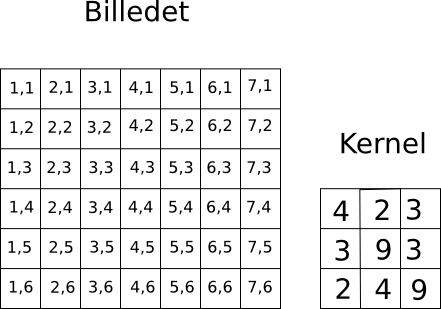
\includegraphics[scale=1,angle=0]{afsnit/vores_implementation/billeder/sloering/convolution}
	\end{center}
	\caption[]{Et billedet og en kernel}
	\label{Convolution}
\end{figure}

Som man kan se i figur \ref{Convolution} er selve billedet og kernel i
vid forskellige størrelser. Måden Convolution virker på at man
multiplicere kernelen ovenpå de værdiger som ligger rund om den pixel,
som vi gerne vil finde den sløret farve af og tager gennemsnittet af den
værdig, f.eks farven på pixel $(4,4)$, bliver

\begin{equation}
	(4,4) = ((3,3)*4+(4,3)*2+(5,3)*3+(3,4)*3+(4,4)*9+(5,4)*3+(3,5)*2+(4,5)*4+(5,5)*9)*\frac{1}{39} 
\end{equation}

I dette eksempel, er punktet $(5,5)$ og $(4,4)$ vægtet højre i forhold til de andet, så farven vil blive sløret i den retning. Dette skyldes at kernelen er bygget tilfældig op, i en rigtige sløring er kernelen meget specifikt udvalgt for at give det beste resultat.
 
\subsubsection*{Gaussian kernel}
Måde Gaussisk sløring bygger sin kernel op på, at ved brug af Gaussian
fordelings formlen, som bliver brugt utallige steder i den matematiske
verden, som en anderkedt og respektere fordelings metode. XXX(ved ikke
om jeg skal komme ind på selve gaussan fordelige, da dette snilt kan
komme op på den del)


\begin{equation}
	G(x,y) = \frac{1}{2\pi\sigma^2}e^{-\frac{x^2+y^2}{2\sigma^2}}
\end{equation}

Hvis $\sigma = 1$ og vi lader x og y køre fra -2 til 2, med steps size på 1, og multiplicere så den laveste værdig kommer til at være 1 og runder værdien af. Få vi en kernel, se firgur \ref{gauss}.

\begin{figure}[h]
	\begin{center}
		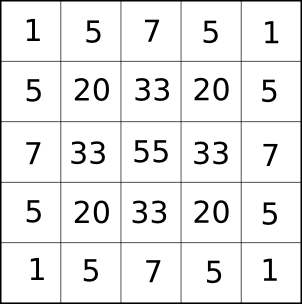
\includegraphics[scale=0.5,angle=0]{afsnit/vores_implementation/billeder/sloering/gauss}
	\end{center}
	\caption[]{Kernel for gauss sløring}
	\label{gauss}
\end{figure}

Denne kernel kan så bruges ved hjælp af concolution til at danne det sløret billet, som vi kan se i figur \ref{gaussian_metode}

\subsubsection*{Sløring ved statistisk median}
Den sidste metode vi vil nævne er i grunden meget simpel. Grundidéen er
at finde den statistiske median i pixelværdierne rundt om en givet pixel
og tildele medianværdien til denne. Givet et antal pixels, er det
trivielt at sætte dem i en liste og sortere dem efter deres værdi. Hvis
antallet af elementer i listen er ulige, er det midterste element i den
sorterede liste medianen. Er der et lige antal elementer i listen,
defineres medianen som gennemsnittet af de to midterste elementer.
Pixels vælges i et $N \times M$ vindue med den originale pixel i
centrum, som vist i figur \ref{red_box_nxm} og vi vil således altid have
et ulige antal elementer i listen.

\begin{figure}[!h]
    \centering
    \subfloat[]{\label{red_box_nxm}
        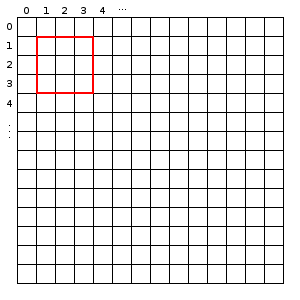
\includegraphics[scale=0.42,angle=0]{afsnit/vores_implementation/billeder/sloering/red_pixel_box}
    }\\
    \subfloat[]{\label{3_3_vindue}
        \renewcommand{\arraystretch}{1.8}
        \begin{tabular}{|c|c|c|}
            \hline
            35 & 98  & 23 \\\hline
            48 & \cellcolor[gray]{0.5}42 & 0 \\\hline
            8  & 12   & 29 \\\hline
        \end{tabular}
        }\hspace{1em}
    \subfloat[]{\label{sorteret_median}
        \renewcommand{\arraystretch}{1.5}
        \centering
        \begin{tabular}{|c|c|c|c|c|c|c|c|c|}
            \hline
            0 & 8 & 12 & 23 & \cellcolor[gray]{0.5}29 & 35 & 42 & 48 & 98\\\hline
        \end{tabular}
        }
        \caption[]{
            Bestemmelse af median for pixel med koordinaterne $(2, 2)$.
            \textbf{\ref{red_box_nxm})} Pixels i et $3\times3$ vindue
            omkring $(2, 2)$ er markeret med rødt.
            \textbf{\ref{3_3_vindue})} Værdierne i $3\times3$ vinduet.
            Det ses den originale pixel har værdien $42$.
            \textbf{\ref{sorteret_median})} Den sorterede liste med
            værdierne fra vinduet. Det ses at medianen har værdien
            $29$. Den originale pixel vil da skifte værdi fra $42$ til
            $29$.
        }
\end{figure}

Denne metode kan ikke køres direkte på det originale billede, da dette
vil interferere med fastsættelse af medianen for alle pixels. Man må
derfor oprette en kopi af det originale billede og sætte de fundne
medianværdier i denne. Man finder således altid medianen i forhold til det
originale billede.

\subsubsection*{Eksempler}

% Hold on, this is figure-madness
\begin{figure}[!h]
    \centering
    \subfloat[Original]{\label{simple_original}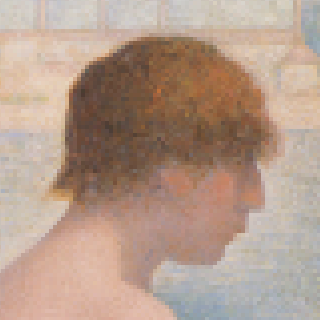
\includegraphics[angle=0,width=0.3\textwidth]{afsnit/vores_implementation/billeder/sloering/original}}\hspace{1em}
    \subfloat[$3 \times 3$ vindue]{\label{simple_3_3}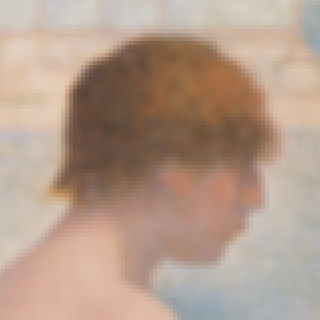
\includegraphics[angle=0,width=0.3\textwidth]{afsnit/vores_implementation/billeder/sloering/simple_3_3}}\hspace{1em}
    \subfloat[$7 \times 7$ vindue]{\label{simple_7_7}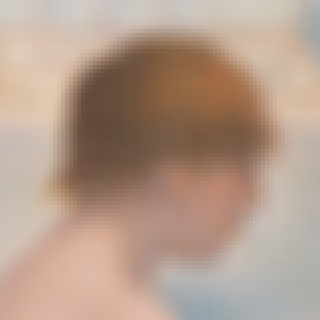
\includegraphics[angle=0,width=0.3\textwidth]{afsnit/vores_implementation/billeder/sloering/simple_7_7}}
    \caption[]{
        \textbf{\ref{simple_original})} Zoom af detajler i det originale billede.
        \textbf{\ref{simple_3_3})}
        \textbf{\ref{simple_7_7})}
    }
    \label{simple_metode}
\end{figure}

\begin{figure}[!h]
    \centering
    \subfloat[Original]{\label{gaussian_original}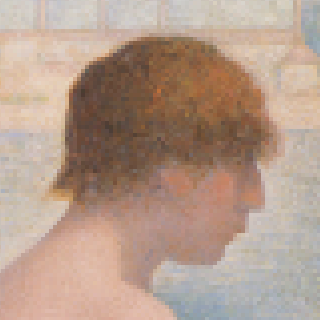
\includegraphics[angle=0,width=0.3\textwidth]{afsnit/vores_implementation/billeder/sloering/original}}\hspace{1em}
    \subfloat[$3 \times 3$ vindue]{\label{gaussian_3_3}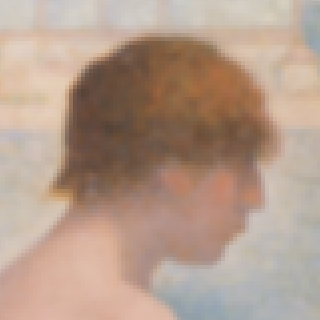
\includegraphics[angle=0,width=0.3\textwidth]{afsnit/vores_implementation/billeder/sloering/gaussian_3_3}}\hspace{1em}
    \subfloat[$7 \times 7$ vindue]{\label{gaussian_7_7}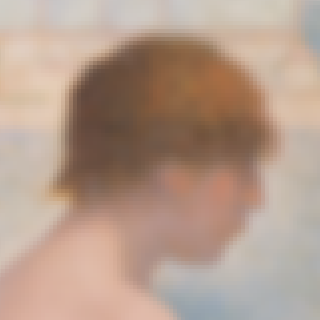
\includegraphics[angle=0,width=0.3\textwidth]{afsnit/vores_implementation/billeder/sloering/gaussian_7_7}}
    \caption[]{
        \textbf{\ref{gaussian_original})} Zoom af detajler i det originale billede.
        \textbf{\ref{gaussian_3_3})}
        \textbf{\ref{gaussian_7_7})}
    }
    \label{gaussian_metode}
\end{figure}

\begin{figure}[!h]
    \centering
    \subfloat[Original]{\label{median_original}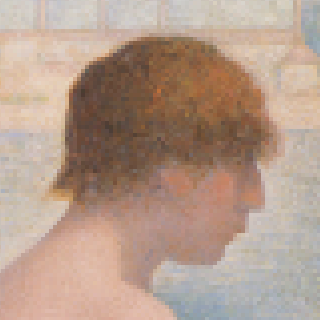
\includegraphics[angle=0,width=0.3\textwidth]{afsnit/vores_implementation/billeder/sloering/original}}\hspace{1em}
    \subfloat[$3 \times 3$ vindue]{\label{median_3_3}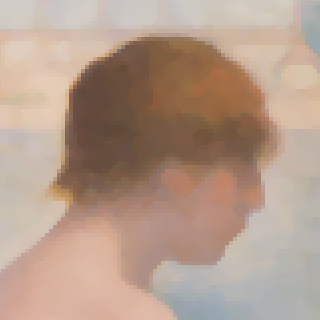
\includegraphics[angle=0,width=0.3\textwidth]{afsnit/vores_implementation/billeder/sloering/median_3_3}}\hspace{1em}
    \subfloat[$7 \times 7$ vindue]{\label{median_7_7}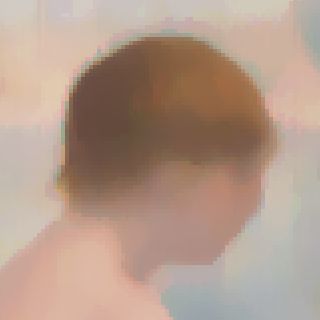
\includegraphics[angle=0,width=0.3\textwidth]{afsnit/vores_implementation/billeder/sloering/median_7_7}}
    \caption[]{
        \textbf{\ref{median_original})} Zoom af detajler i det originale billede.
        \textbf{\ref{median_3_3})} Median med et vindue på $3\times{}3$.
        Farverne er blevet mere ensartede mens kanterne stadig er
        skarpe.
        \textbf{\ref{median_7_7})} Median med et vindue på $7\times{}7$. Farverne
        er meget ensartede, men det ses at kanterne er blevet mere
        udvisket med det større vindue.
    }
    \label{median_metode}
\end{figure}

}

% vim: set tw=72 spell spelllang=da:
